%!TEX root = ../thesis.tex

\chapter{Data} \label{ch:data}

\newthought{In order to carry out the analysis herein,} it was necessary to gather
play-by-play data with complete lineups. To do this, I collected play-by-play data
from the past eleven completed NBA seasons, starting with the 2005-06 season and
ending with the 2015-16 season. The data was scraped from \citet{BKRef}; this site
was chosen for several reasons. First, the website makes its data freely available
and is organized simply and effectively, simplifying the scraping process.  The
second and more important reason the site was chosen is because it assigns unique
identifiers to each entity for which it has data, including players, teams, seasons,
coaches, and referees. Using these unique identifiers, it is very easy to
cross-reference and join different data sources from the site; this makes complex
analyses simpler because there it eliminates guesswork and ambiguities in data
wrangling. For example, while other data sources may have ambiguities arising from
players with similar names, Basketball Reference's unique identifiers make it easy
to distinguish between, for example, Tim Hardaway Jr. and Tim Hardaway Sr. or Isiah
Thomas and Isaiah Thomas.

The data scraping was done in Python using the sportsref library, an open-source
Python library for scraping sports data from Basketball Reference and its sister
sites, which include Pro Football Reference and Baseball Reference, among others. I
am the sole creator, developer, and maintainer of the library, which was
created to make sports analytics easier for those who understand sports and basic
data analysis but do not have the programming knowledge to scrape data themselves.
The library is still in the early stages of development; its code can be found on
GitHub \cite{Sportsref}.

More specifically, the data used in this thesis was scraped from the play-by-play
section that Basketball Reference provides for virtually every game since the
beginning of the 2000-2001 NBA season. For an example of what this looks like, see
figure~\ref{fig:bkref_pbp}. This page gives detailed text descriptions of each event
throughout the game, but does not contain structured data to identify, for example,
whether an event is a rebound or who the shooter is on a field goal attempt.
Therefore, regular expressions were constructed for each type of event in the
dataset in order to create structured data from these descriptions; altogether,
there are about twenty different types of events.

\begin{figure}
    \centering
    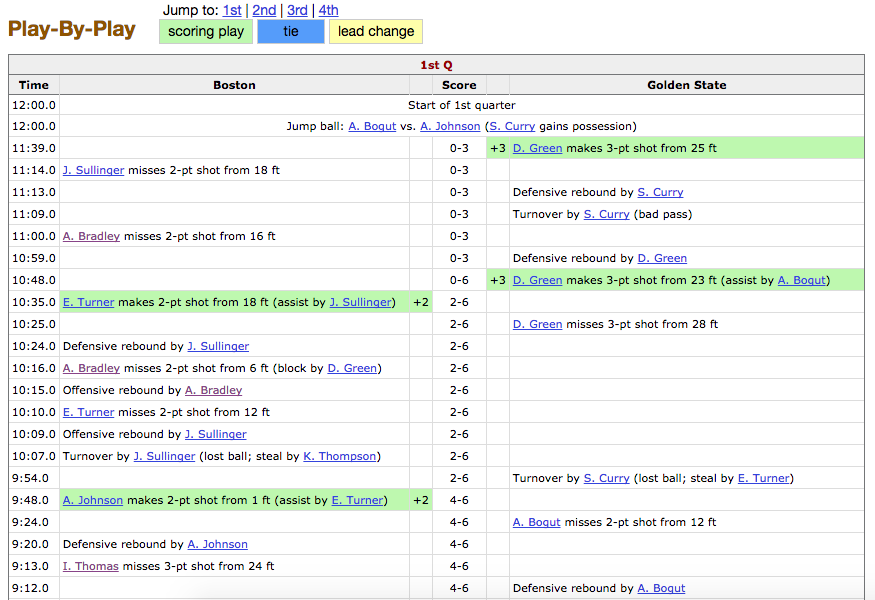
\includegraphics[width=\textwidth]{figures/bkref_pbp}
    \caption{An example of the Basketball Reference play-by-play source for a
    Warriors-Celtics game in April 2016.}
    \label{fig:bkref_pbp}
\end{figure}

Moreover, several issues exist in the raw data that required cleaning. Perhaps the
most difficult problem with the raw data is that some events were ordered
incorrectly. Examples include rebounds being listed prior to their corresponding
missed shots and inconsistencies surrounding when substitutions and timeouts occur
during free throws; these problems were remedied by a complicated sorting scheme
within each possession so that events were listed in a logical order. Other,
slightly simpler problems included tracking which team was on offense or defense at
any given time and consolidating redundant substutitions in which a player would sub
in and immediately sub out.

Once the raw data was cleaned, additional features were added to the data. For
instance, simple new features include the home and away teams' points scored on each
event, which can be used to easily compute point differential for any subset of
events. One very important and more complicated feature was identifying ``plays,'' a
possession-like concept introduced by \citeauthor{Maymin} In particular, the
definition of a play is identical to the definition of a possession, except that an
offensive rebound extends a possession but begins a new play. Distinguishing plays
from possessions was important because it provides more context for the profile
statistics described in section \ref{sec:profiles}, as each play allows another
opportunity to log events such as field goal attempts, rebounds, assists, and
personal fouls. Therefore, when computing rate statistics for players, it is more
revealing to use per-play statistics than per-possession statistics.
Differentiating plays was done by labeling events that end a play with an indicator
variable and computing the cumulative sum of these variables to create a play
identification number for each event. Specifically, play-ending events include
turnovers, field goal attempts on which fouls were not committed, free throws that
are not succeeded by another free throw, and the end of each quarter or overtime
period. Possessions were identified using a similar procedure; while plays are more
indicative of play style for most of the profile statistics in section
\ref{sec:profiles}, others (in particular, RAPM) require possession data. Moreover,
throughout the analysis herein, technical fouls and technical free throws were
discarded from the play-by-play data set, as they sometimes caused issues when
identifying plays and possessions and are generally rare enough that they can be
safely ignored for the sake of this analysis.

Next, analyzing lineups requires data that indicates which players are on the court
for any given event. While the data provided by basketball-reference.com does not
explicitly give this information, it does include substitution data, where each
substitution is logged as an independent event. However, substitution events are
only logged for substitutions in the middle of a quarter or overtime period;
substitutions between periods were not indicated in the raw data. Therefore, to
determine which players start each period, it was necessary to comb through each
period and note which players are involved in events (including being substituted
out) prior to being substituted in. When a player who started a period was never
substituted out and was never involved in an event, the player can be determined by
computing each player's minutes played based on the play-by-play data and comparing
this value to his minutes played as listed in the box score. Once the starters of
each period were determined, it is relatively straightforward to use substitution
data to determine each team's lineup for any given event.

\begin{table}
    \centering
    \noindent\makebox[\textwidth]{%
\begin{tabular}{cccccc}
\toprule
  boxscore\_id &  secs\_elapsed &  poss\_id & off\_team & def\_team &                        detail \\
\midrule
 201604050SAC &        2416.0 &   222933 &      SAC &      POR &                 couside01 misses free throw 1 of 1 \\
 201602280DAL &        2440.0 &   168496 &      DAL &      MIN &               bareajo01 misses 2-pt shot from 4 ft \\
 201512050TOR &        1358.0 &    57123 &      TOR &      GSW &  Personal take foul by ezelife01 (drawn by jose... \\
 201511290NYK &         918.0 &    48221 &      NYK &      HOU &  willide02 makes 2-pt shot at rim (assist by ga... \\
 201511070SAS &        2229.0 &    17897 &      CHO &      SAS &                     Defensive rebound by millspa02 \\
 201601040PHI &        1807.0 &    99151 &      MIN &      PHI &                      Defensive rebound by noelne01 \\
 201512090BOS &        1534.0 &    61355 &      CHI &      BOS &  gibsota01 misses 2-pt shot from 1 ft (block by... \\
 201512100CHI &        1108.0 &    63424 &      LAC &      CHI &                  redicjj01 makes free throw 2 of 2 \\
 201601290MIL &         453.0 &   133985 &      MIA &      MIL &            bayleje01 enters the game for antetgi01 \\
 201511110SAC &        2003.0 &    23768 &      DET &      SAC &              johnsst04 misses 3-pt shot from 24 ft \\
 201512050PHI &        2794.0 &    56839 &      PHI &      DEN &            stausni01 enters the game for mccontj01 \\
 201603120PHI &        2122.0 &   187975 &      PHI &      DET &                  stausni01 makes free throw 1 of 2 \\
 201603040BOS &         440.0 &   174876 &      BOS &      NYK &                     Defensive rebound by thomala01 \\
 201601300NOP &        1384.0 &   135784 &      BRK &      NOP &                 lopezbr01 misses free throw 1 of 2 \\
 201510300ORL &         774.0 &     5375 &      ORL &      OKC &                  fournev01 makes free throw 1 of 1 \\
 201511110ATL &        1271.0 &    21868 &      ATL &      NOP & New Orleans full timeout \\
 201601030WAS &         474.0 &    97574 &      WAS &      MIA &                     Offensive rebound by gortama01 \\
 201511190CLE &        1789.0 &    33784 &      MIL &      CLE &  antetgi01 makes 2-pt shot at rim (assist by pa... \\
 201603150IND &         388.0 &   191471 &      IND &      BOS &                  Turnover by stuckro01 (traveling) \\
 201602010SAC &        2153.0 &   138904 &      SAC &      MIL &                       Offensive rebound by acyqu01 \\
\bottomrule
\end{tabular}
    }
    \caption{An example of events logged in the play-by-play data.}
    \label{tab:pbp}
\end{table}

It is important to note that Basketball Reference's play-by-play is not official,
and in some cases there was missing data. For the seasons being used here,
play-by-play was available for every game, but there were errors in parsing the raw
data in four games out of the 13,289 games ($0.03\%$) played during the
eleven-season span; all of these errors were caused by inconsistent or insufficient
substitution data in the play-by-play logs, resulting in an inability to determine
the players on the court for at least one event in the play-by-play. These games
were simply ignored for the sake of this analysis. Moreover, in order to ensure that
the data was by-and-large accurate, each player's raw plus/minus was calculated in
each remaining game based on the lineup data inferred from the play-by-play and
compared to the raw plus/minus listed in the box score summary provided by
Basketball Reference. For 91.6\% of the games for which there is complete data,
there was no difference between any player's computed plus/minus and his official
plus/minus. In 99.4\% of the games, there is no absolute difference between the
plus/minus figures that exceeds two points. Finally, in 99.91\% of the games, the
sum of all players' computed plus/minus was equal to zero, which is a necessary
condition of correct raw plus/minus data within a game. These figures suggest that
the vast majority of the data is correct and can be trusted with reasonably high
confidence.
